\documentclass{article}
\usepackage[utf8]{inputenc}

\usepackage{amsthm}
\usepackage{amsmath}
\usepackage{amssymb}
\usepackage{xcolor}
\usepackage{tikz}
\usepackage{bbm}
\usepackage{pgfplots}
\usepackage{caption}
\usepackage{subcaption}

\usetikzlibrary{patterns}

\DeclareMathOperator{\err}{err}

\theoremstyle{plain}
\newtheorem{thrm}{Théorème}[section]
\newtheorem{lem}[thrm]{Lemme}
\newtheorem{prop}[thrm]{Proposition}

\theoremstyle{remark}
\newtheorem{rem}[thrm]{Remarque}
\newtheorem{exmp}[thrm]{Exemple}

\theoremstyle{definition}
\newtheorem{defin}[thrm]{Définition}

\title{Apprentissage (Machine learning)}
\author{Notes par Sarah Vita Paardekooper}
\date{08 Octobre 2020}

\begin{document}

\maketitle

\setcounter{section}{2}

\section{Agnostic setting}


Soient $X$ un domaine, $Y$ un ensemble d'étiquettes et $\mathcal{H}\subset \{f : X \rightarrow Y \}$ un ensemble d'hypothèses.

Dans le modèle de cohérence (consistency model), on suppose qu'il existe un $c\in\mathcal{H}$ tel que l'échantillon $S$ est cohérent avec $c$, c'est à dire $S=\{(x_i,c(x_i))\}_i$. L'objectif est donc de trouver une hypothèse $h\in \mathcal{H}$ cohérent avec $S$.

Dans le modèle PAC, on suppose qu'il existe un $c\in\mathcal{H}$ tel que l'échantillon $S$ est cohérent avec $c$, c'est à dire $S=\{(x_i,c(x_i))\}_i$. Mais on suppose que les $x_i$ peuvent contenir du bruit, donc on suppose une distribution $\mathcal{D}$ sur le domaine $X$ et $S$ suit $\mathcal{D}^m$. L'objectif est donc de trouver une hypothèse $h\in\mathcal{H}$ tel que $\mathbb{P}_{S\sim \mathcal{D}^m}(\err_c(h)\leq \epsilon)\geq 1-\delta$ où $\err_c(h)=\mathbb{P}_{X\sim\mathcal{D}}(h(x)=c(x))$.

Dans le modèle PAC agnostic, on suppose l'existence de bruit sur le domaine ainsi que sur les étiquettes, c'est à dire une distribution $\mathcal{D}$ sur $X\times Y$. L'échantillon $S=\{(x_i,y_i)\}_i$ suit alors une distribution $\mathcal{D}^m$. Dans ce modèle, l'objectif est de trouver $h\in\mathcal{H}$ tel que 
$$ \mathbb{P}_{S\sim\mathcal{D}^m} (\err(h)-\inf_{h'\in\mathcal{H}} \err(h')\leq \epsilon ) \geq 1- \delta $$
où $\err(h)=\mathbb{P}_{(X,Y)\sim\mathcal{D}} (h(x)\neq y)$.

L'\textbf{erreur empirique} est définit par $\widehat{\err}(h)= \frac{1}{m} \sum\limits_{i=1}^{m} \mathbbm{1}_{h(x_i)\neq y_i}$, pour $h\in\mathcal{H}$.

\begin{defin}
    On dit que $h_{ERM}\in \mathcal{H}$ est une hypothèse \textbf{ERM} (Empirical Risk Minimisation) si $\widehat{\err}(h_{ERM})= \min_{h\in \mathcal{H}} \widehat{\err}(h)$, c'est à dire si
    $$ h_{ERM}= \arg \min_{h\in \mathcal{H}} \widehat{\err}(h) .$$
    Un algorithme est \textbf{ERM} s'il retourne une hypothèse ERM.
\end{defin}

\begin{defin}
    On dit que $\mathcal{H}$ est \textbf{apprenable au sens agnostic PAC} s'il existe un algorithme calculant une hypothèse $h$ tel que $ \forall\epsilon , \forall\delta , \forall\mathcal{D} \text{ sur } X\times Y, \exists M\in\mathbb{N}, \forall m\geq M,$
    $$ \mathbb{P}_{S\sim\mathcal{D}^m} (\err(h)-\inf_{h'\in\mathcal{H}} \err(h')\leq \epsilon ) \geq 1- \delta $$
\end{defin}

\begin{thrm}
    $\mathcal{H}$ est apprenable au sens agnostic PAC si et seulement si $\mathcal{H}$ a VC-dimension finie.
\end{thrm}

La VC-dimension est une mesure de la capacité d'apprendre un ensemble de fonction par classification statistique binaire.

\begin{defin}
    La Propriété de Convergence Uniforme (\textbf{UCP}) est définit comme suit :
    $$ \forall h\in\mathcal{H}, \mathbb{P}_{(X,Y)\sim\mathcal{D}} (h(x) \neq y) = | \err(h) - \widehat{\err}(h)| \leq \frac{\epsilon}{2} $$
\end{defin}

\begin{lem}
    Si UCP est vraie (pour $\epsilon$ fixéé), alors l'algorithme ERM ayant $h_{ERM}$ en sortie satisfait $\err(h_{ERM}) - \inf_{h\in\mathcal{H}} \err(h) \leq \epsilon$.
\end{lem}

\begin{proof}[Preuve]
Notons $h_{OPT} = \arg\inf_{h\in\mathcal{H}} \err(h)$. Montrons que $\err(h_{ERM})-\err(h_{OPT}) \leq \epsilon$ :\\
$\err(h_{ERM})-\err(h_{OPT}) \leq \underbrace{\err(h_{ERM}) - \widehat{\err}(h_{ERM})}_{\leq \epsilon / 2 \text{ (UCP)}} + \underbrace{\widehat{\err}(h_{ERM})}_{\widehat{\err}(h_{OPT})\text{ (ERM)}} - \err(h_{OPT})$\\
$\phantom{\err(h_{ERM})-\err(h_{OPT})} \leq \frac{\epsilon}{2} + \underbrace{\widehat{\err}(h_{OPT}) - \err(h_{OPT})}_{\leq \epsilon / 2 \text{ (UCP)}}$\\
$\phantom{\err(h_{ERM})-\err(h_{OPT})} \leq \frac{\epsilon}{2} + \frac{\epsilon}{2} = \epsilon $
\end{proof}

Soient un domaine $X$ et un ensemble d'étiquettes $Y=\{0,1\}$. Notons que l'ensemble $\mathcal{H}$ de fonctions $X \rightarrow \{0,1\}$ est équivalent à l'ensemble de sous-ensembles de $X$ (puisque toutes les fonctions peuvent être exprimées sous la forme $\mathbbm{1}_A$, avec $A\subseteq X$).

\begin{defin}
    Soit $S\subseteq X$ un échantillon. On dit que $S$ est \textbf{explosé} (shattered) par $\mathcal{H}$ si $\forall P \subseteq S, \exists h \in \mathcal{H}, \forall x \in S, h(x)=1 \Leftrightarrow x \in P$.
\end{defin}

Exemple : \\
$X=\mathbb{R}^n$, $\mathcal{H}_n = \{f : \mathbb{R}^n \rightarrow \{0,1\} : f(\overrightarrow{x})= 1 \text{ si } \overrightarrow{x} \cdot \overrightarrow{a} \geq b \text{ et 0 si } \overrightarrow{x} \cdot \overrightarrow{a} < b \}$, avec $\overrightarrow{a}\in \mathbb{R}^n$ et $b\in \mathbb{R}$. $\mathcal{H}_n$ est l'ensemble des fonctions dans $\mathbb{R}^n$ définient par un hyperplan, avec tout les points valant 1 d'une part de l'hyperplan, et 0 de l'autre.

\begin{itemize}
    \item n=2 : 
    \begin{itemize}
        \item Si $|S|=2$, $S$ est toujours explosé.        
        \item Il existe des échantillons $S$, $|S|=3$ explosés et il existent des échantillons $S$, $|S|=3$ non explosés.
        \item Tout échantillon $S$, $|S|\geq 4$, est non explosé
    \end{itemize}
\end{itemize}
        
\begin{figure}
\centering
\begin{subfigure}{.24\textwidth}
\centering
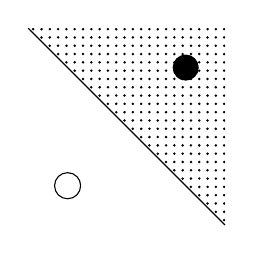
\begin{tikzpicture}
    \node[shape=circle,draw=black] (1) at (0,0) {};
    \path [pattern=dots] (-0.5,2) -- (2,-0.5) -- (2,2) -- (-0.5,2) -- cycle;
    \node[shape=circle,fill=black] (2) at (1.5,1.5) {};
    \path[] (-0.5,2) edge (2,-0.5);
\end{tikzpicture}
\caption{S est explosé}
\end{subfigure}
\begin{subfigure}{.24\textwidth}
\centering
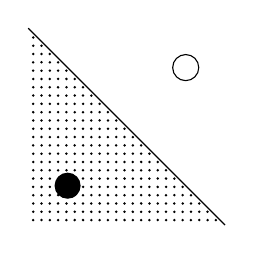
\begin{tikzpicture}
    \path [pattern=dots] (-0.5,2) -- (2,-0.5) -- (-0.5,-0.5) -- (-0.5,2) -- cycle;
    \node[shape=circle,fill=black] (1) at (0,0) {};
    \node[shape=circle,draw=black] (2) at (1.5,1.5) {};
    \path[] (-0.5,2) edge (2,-0.5);
\end{tikzpicture}
\caption{S est explosé}
\end{subfigure}
\begin{subfigure}{.24\textwidth}
\centering
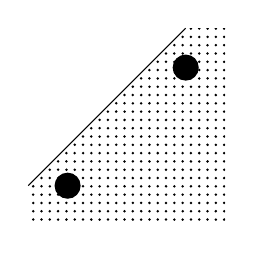
\begin{tikzpicture}
    \path [pattern=dots] (1.5,2) -- (-0.5,0) -- (-0.5,-0.5) -- (2,-0.5) -- (2,2) -- (1.5,2) -- cycle;
    \node[shape=circle,fill=black] (1) at (0,0) {};
    \node[shape=circle,fill=black] (2) at (1.5,1.5) {};
    \path[] (1.5,2) edge (-0.5,0);
\end{tikzpicture}
\caption{S est explosé}
\end{subfigure}
\begin{subfigure}{.24\textwidth}
\centering
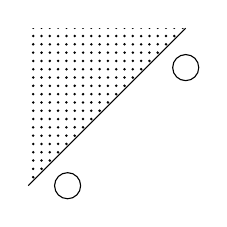
\begin{tikzpicture}
    \path [pattern=dots] (1.5,2) -- (-0.5,0) -- (-0.5,2) -- (1.5,2) -- cycle;
    \node[shape=circle,draw=black] (1) at (0,0) {};
    \node[shape=circle,draw=black] (2) at (1.5,1.5) {};
    \path[] (1.5,2) edge (-0.5,0);
\end{tikzpicture}
\caption{S est explosé}
\end{subfigure}
\\
\begin{subfigure}{.3\textwidth}
\centering
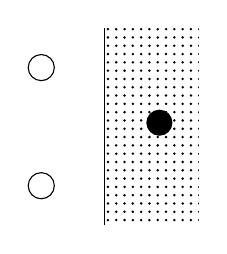
\begin{tikzpicture}
    \path [pattern=dots] (0.8,2) -- (0.8,-0.5) -- (2,-0.5) -- (2,2) -- (0.8,2) -- cycle;
    \node[shape=circle,draw=black] (1) at (0,0) {};
    \node[shape=circle,draw=black] (1) at (0,1.5) {};
    \node[shape=circle,fill=black] (2) at (1.5,0.8) {};
    \path[] (0.8,2) edge (0.8,-0.5);
\end{tikzpicture}
\caption{S est explosé}
\end{subfigure}
\begin{subfigure}{.3\textwidth}
\centering
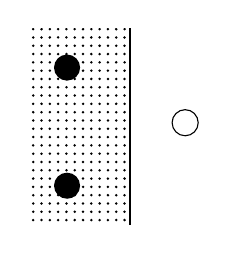
\begin{tikzpicture}
    \path [pattern=dots] (0.8,2) -- (0.8,-0.5) -- (-0.5,-0.5) -- (-0.5,2) -- (0.8,2) -- cycle;
    \node[shape=circle,fill=black] (1) at (0,0) {};
    \node[shape=circle,fill=black] (1) at (0,1.5) {};
    \node[shape=circle,draw=black] (2) at (1.5,0.8) {};
    \path[] (0.8,2) edge (0.8,-0.5);
\end{tikzpicture}
\caption{S est explosé}
\end{subfigure}
\begin{subfigure}{.3\textwidth}
\centering
\begin{tikzpicture}
    \node[shape=circle,draw=black] (1) at (0,0) {};
    \node[shape=circle,draw=black] (2) at (2,2) {};
    \node[shape=circle,fill=black] (3) at (1,1) {};
\end{tikzpicture}
\caption{S n'est pas explosé}
\end{subfigure}
\caption{Les points noirs sont dans $P$, et la zone en pointillés vaut 1.}
\end{figure}

\begin{defin}
    On définit alors la \textbf{VC-dimension} comme $$\text{VCdim}(\mathcal{H}) = \max \{ |S| : S \text{ explosé par } \mathcal{H} \}$$
\end{defin}

Exemples : $\text{VCdim}(\mathcal{H}_2) = 3$, $\text{VCdim}(\mathcal{H}_n) = n+1$. $X=\mathbb{N}$, $\mathcal{H}$ est l'ensemble de toutes les fonctions, $\text{VCdim}(\mathcal{H}) = \infty $.

\begin{defin}
    La \textbf{fonction de croissance} de $\mathcal{H}$ est définit par
    \begin{align*}
        \Pi_\mathcal{H} : & \mathbb{N} \rightarrow \mathbb{N}\\
        & m \mapsto \max_{S\subseteq X, |S|=m} |\{h|_S : h\in \mathcal{H}\} |
    \end{align*}
\end{defin}

\begin{rem}
    Pour $\text{VCdim}(\mathcal{H}) = d$, on a $\Pi_\mathcal{H}(d+1)<2^{d+1}$, $\Pi_\mathcal{H}(d)=2^d$, et $\Pi_\mathcal{H}(d')=2^{d'}$ pour tout $d'\leq d$.
    
    On a aussi que $S$ est explosé par $\mathcal{H}$ si et seulement si $|\{h|_S : h\in \mathcal{H}\} |=2^d$.
\end{rem}

\begin{lem}(Sauer)
    Si $\text{VCdim}(\mathcal{H}) = d$, alors $$\Pi_\mathcal{H}(m) \leq \sum\limits_{i=0}^d {m\choose i} \leq \left ( \frac{e m}{d} \right )^d = O(m^d) .$$
\end{lem}

\end{document}
